CLEO cones, used by the CLEO collaboration and introduced in Ref.~\cite{CLEO:1995rok}, are defined accordingly to momentum flow around an axis $\vec{A}$.
Nine cones are defined, with opening angles between 10 and 90 degrees. 
The energy flux in all of them is measured.
Spherical decays tend to have their energy distributed more equally amongst the cones, whereas collinear decays have most of the energy within the first few.
In this analysis, 18 CLEO cones are tested: 9 defined with respect to the event thrust axis, $\mathtt{CC}_{i}$, and 9 defined with respect to the tag-side $B$ meson thrust axis, $\mathtt{CC}^B_{i}$.
The results for \textbf{Test~1} are shown in \Cref{fig:Btag_CleoCone0,fig:Btag_CleoCone1,fig:Btag_CleoCone2,fig:Btag_CleoCone3,fig:Btag_CleoCone4,fig:Btag_CleoCone5,fig:Btag_CleoCone6,fig:Btag_CleoCone7,fig:Btag_CleoCone8,fig:cleoConeThrust0,fig:cleoConeThrust1,fig:cleoConeThrust2,fig:cleoConeThrust3,fig:cleoConeThrust4,fig:cleoConeThrust5,fig:cleoConeThrust6,fig:cleoConeThrust7,fig:cleoConeThrust8}.
Outermost cones, generally, show a higher degree of correlation with \EB, \Estar and \Mbc, and only 6 CLEO cones with an opening angle of up to 30 degrees pass the test.

\begin{figure}[htbp!]
    \centering
    \subcaptionbox{\label{fig:Btag_CleoCone0}}{
        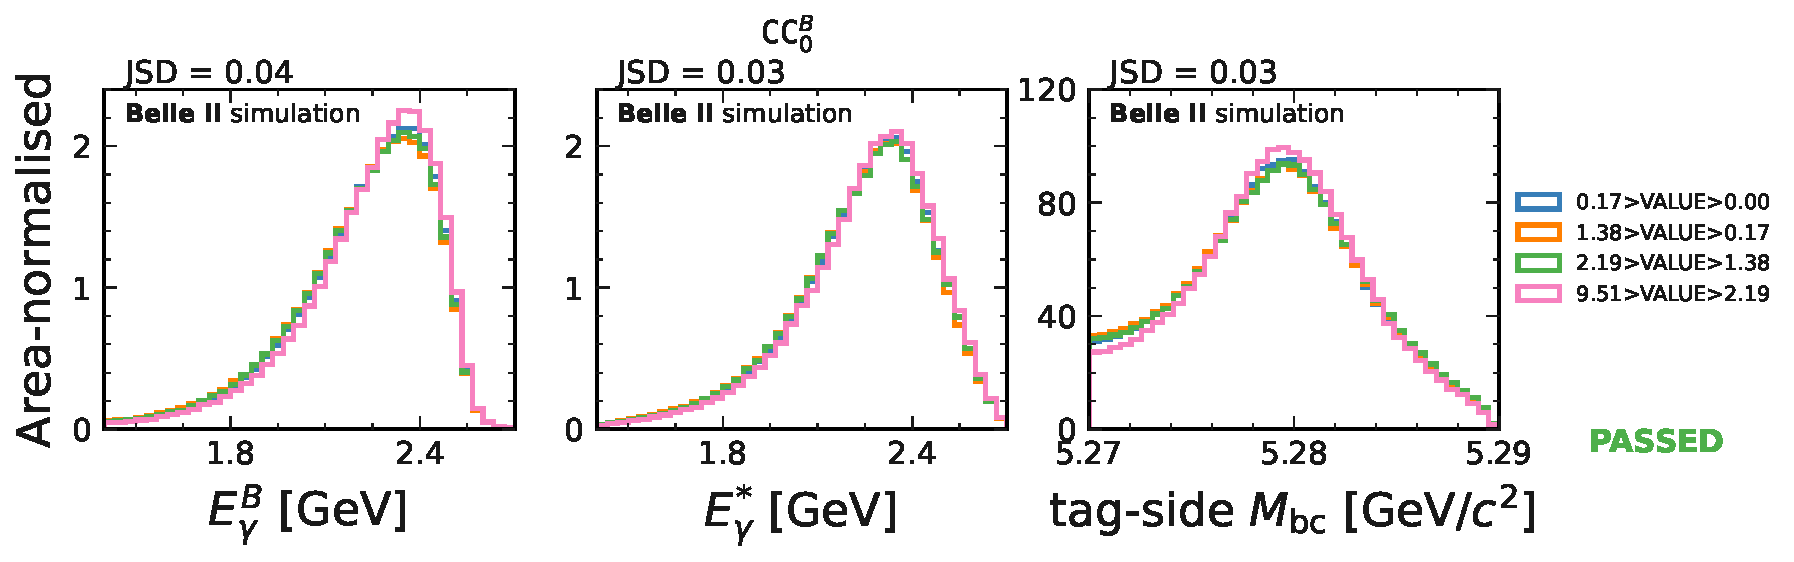
\includegraphics[width=0.95\textwidth]{figures/appendices/continuum_suppression_features/cleo_cones/Btag_CleoCone1_bias_tested.pdf}
    }
    \subcaptionbox{\label{fig:Btag_CleoCone1}}{
        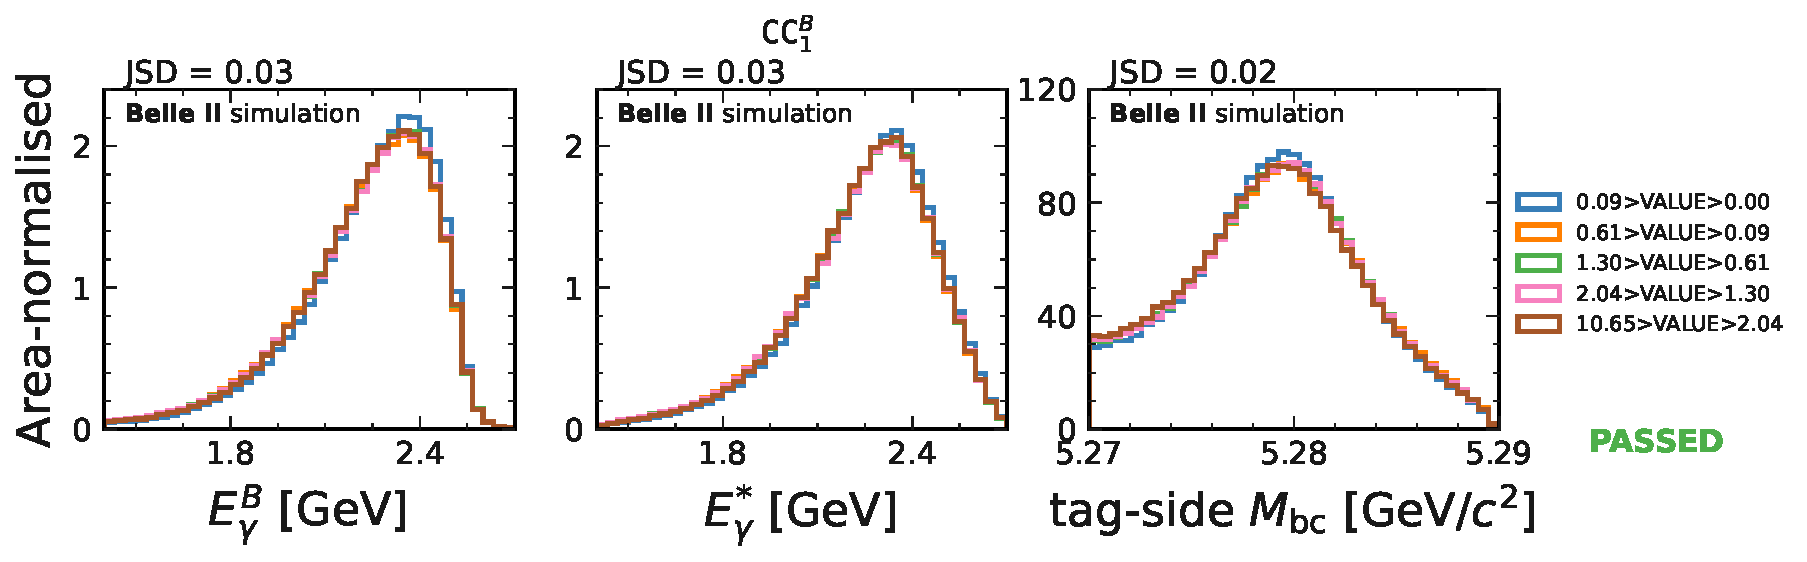
\includegraphics[width=0.95\textwidth]{figures/appendices/continuum_suppression_features/cleo_cones/Btag_CleoCone2_bias_tested.pdf}
    }
    \subcaptionbox{\label{fig:Btag_CleoCone2}}{
        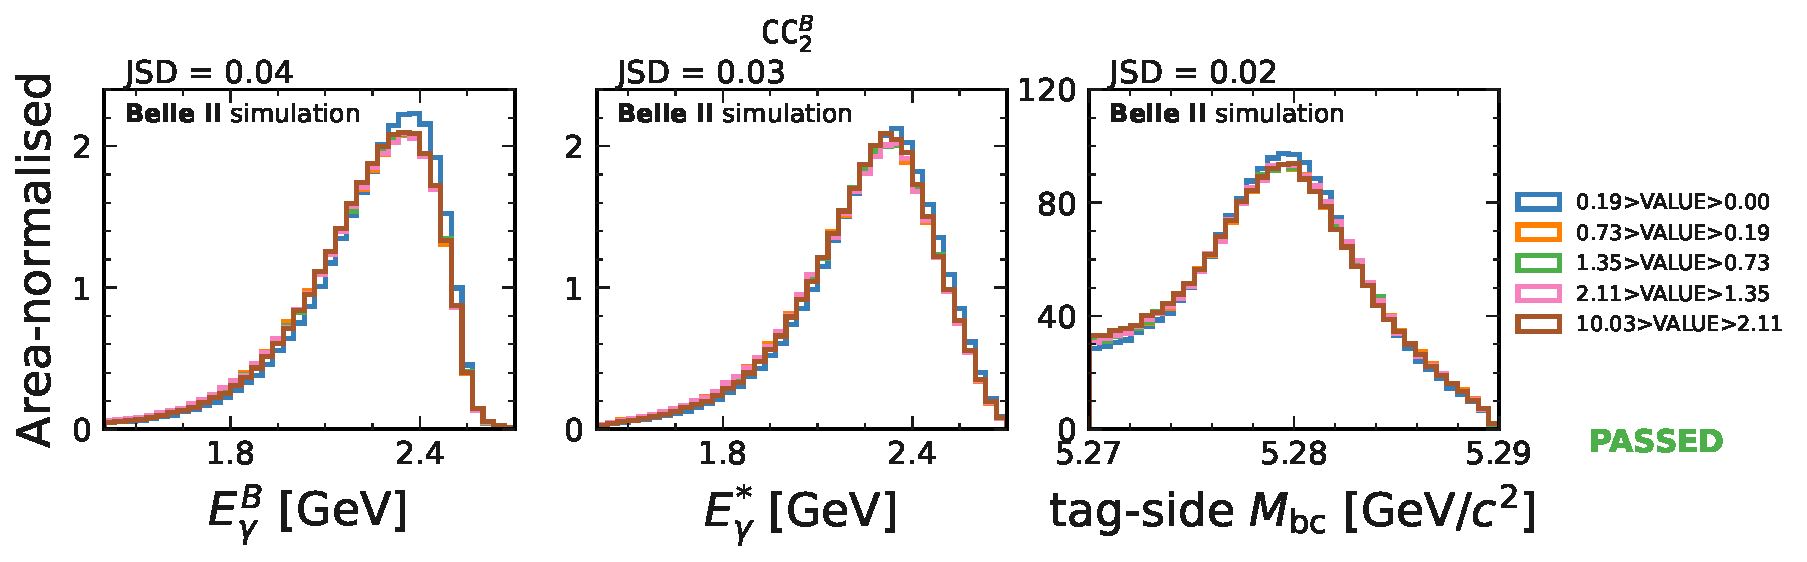
\includegraphics[width=0.95\textwidth]{figures/appendices/continuum_suppression_features/cleo_cones/Btag_CleoCone3_bias_tested.pdf}

    }
    \subcaptionbox{\label{fig:Btag_CleoCone3}}{
        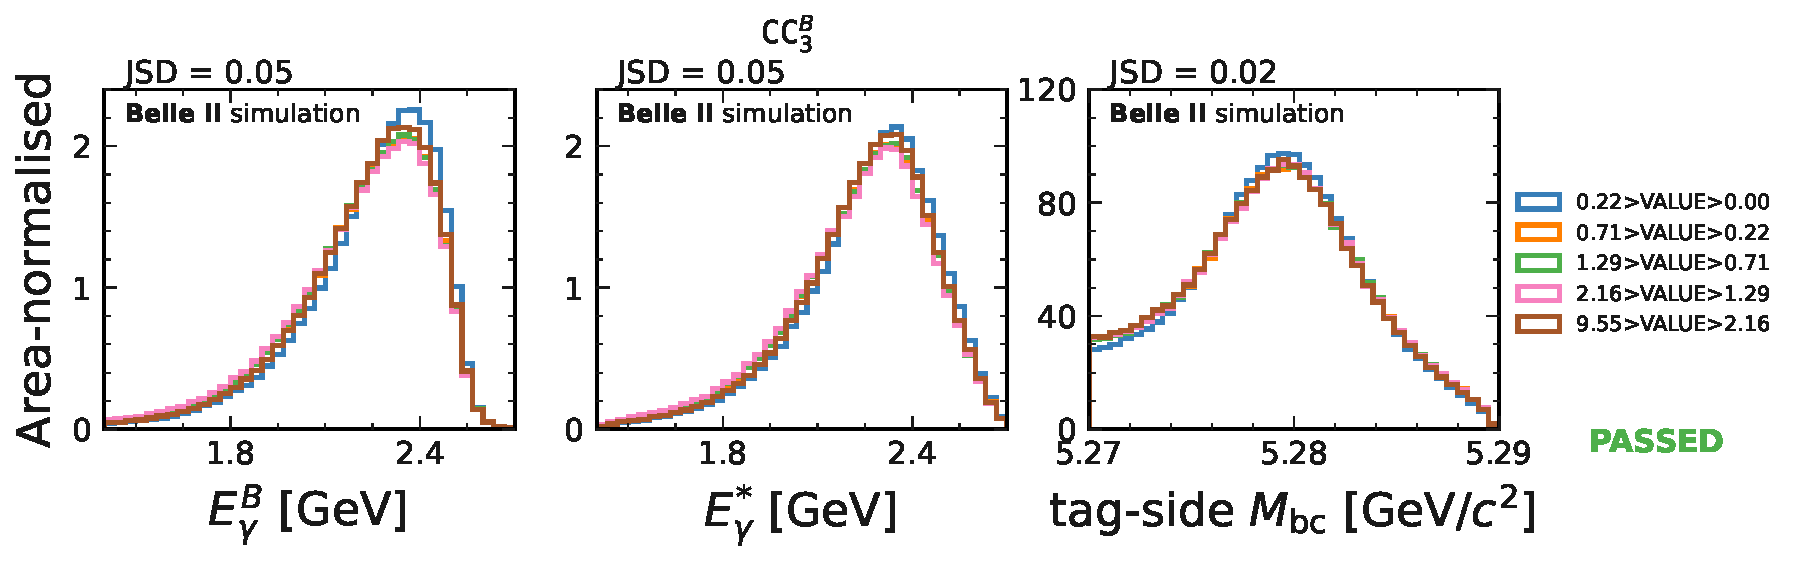
\includegraphics[width=0.94\textwidth]{figures/appendices/continuum_suppression_features/cleo_cones/Btag_CleoCone4_bias_tested.pdf}

    }
\end{figure}
\begin{figure}[htbp!]
    \centering
    \ContinuedFloat
    \subcaptionbox{\label{fig:Btag_CleoCone4}}{
        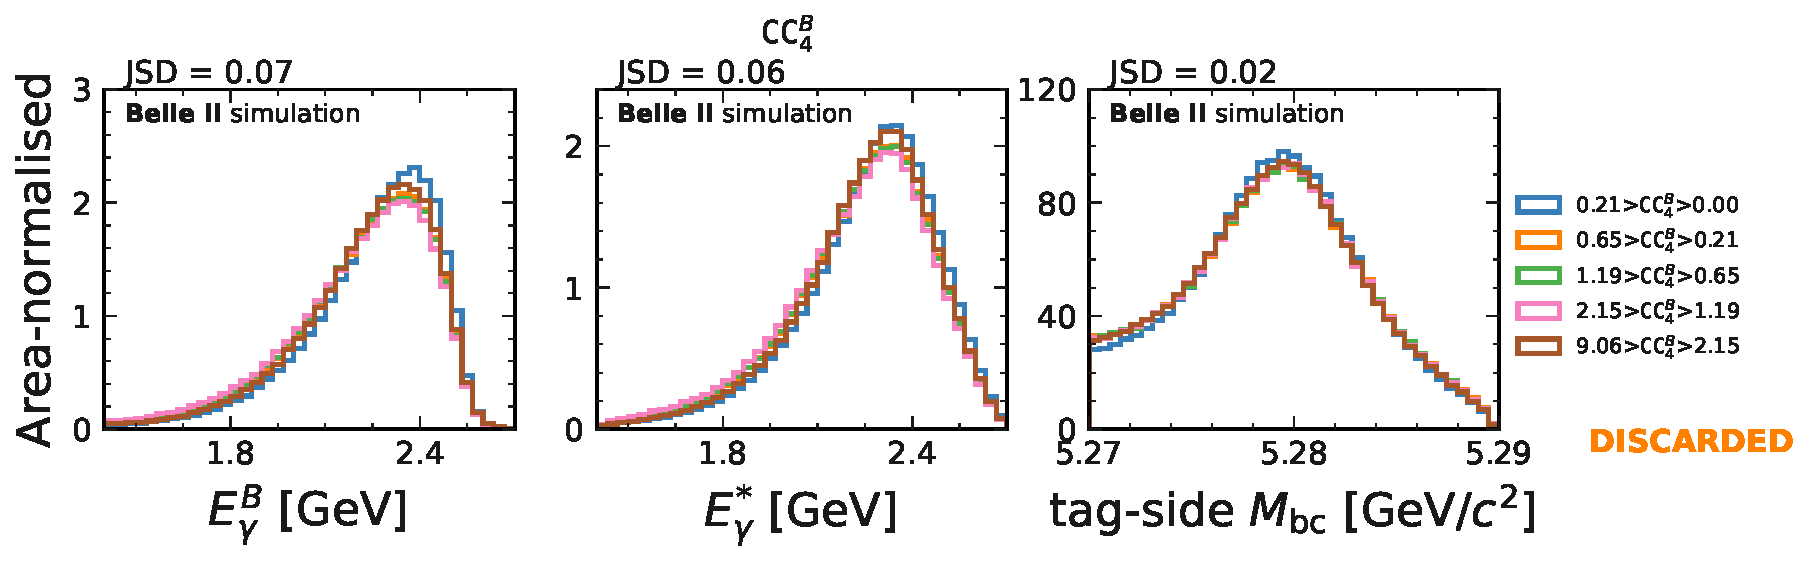
\includegraphics[width=0.95\textwidth]{figures/appendices/continuum_suppression_features/cleo_cones/Btag_CleoCone5_bias_tested.pdf}

    }
    \subcaptionbox{\label{fig:Btag_CleoCone5}}{
        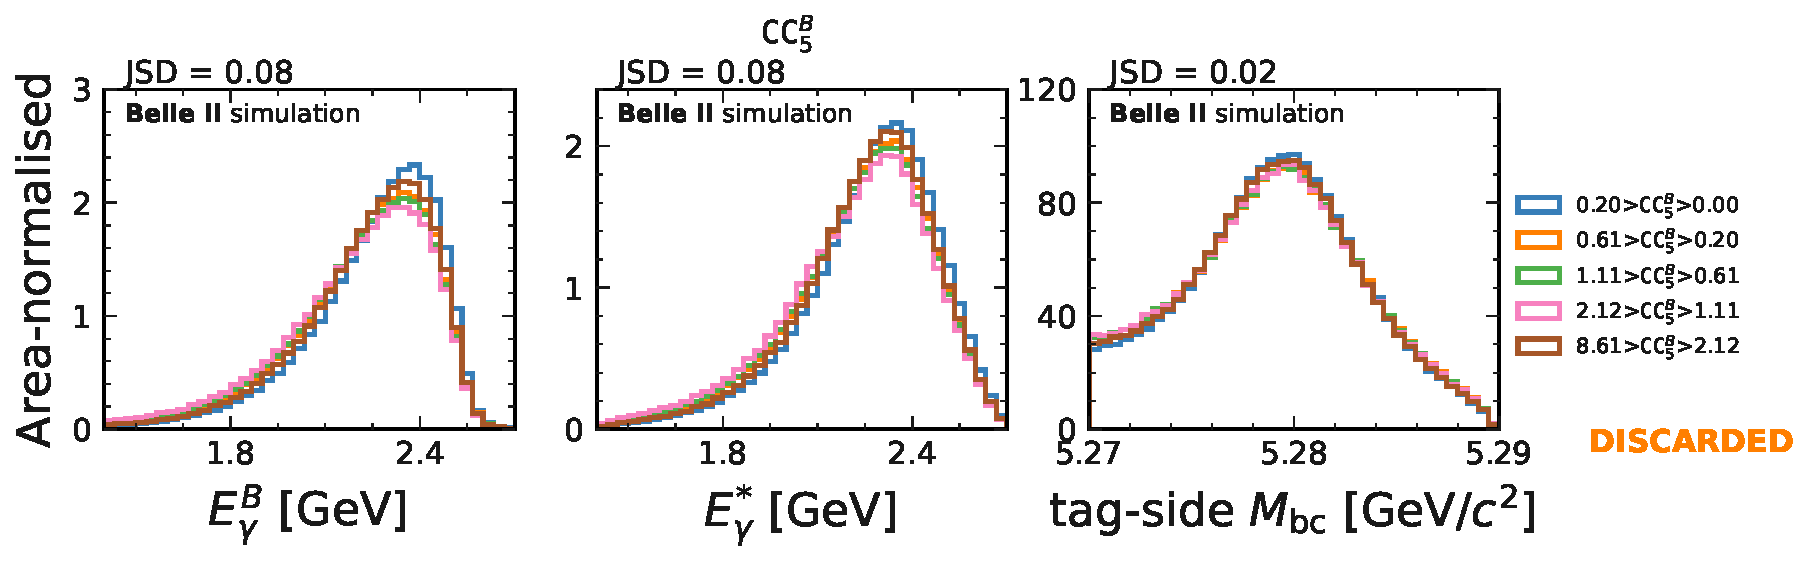
\includegraphics[width=0.95\textwidth]{figures/appendices/continuum_suppression_features/cleo_cones/Btag_CleoCone6_bias_tested.pdf}

    }
    \subcaptionbox{\label{fig:Btag_CleoCone6}}{
        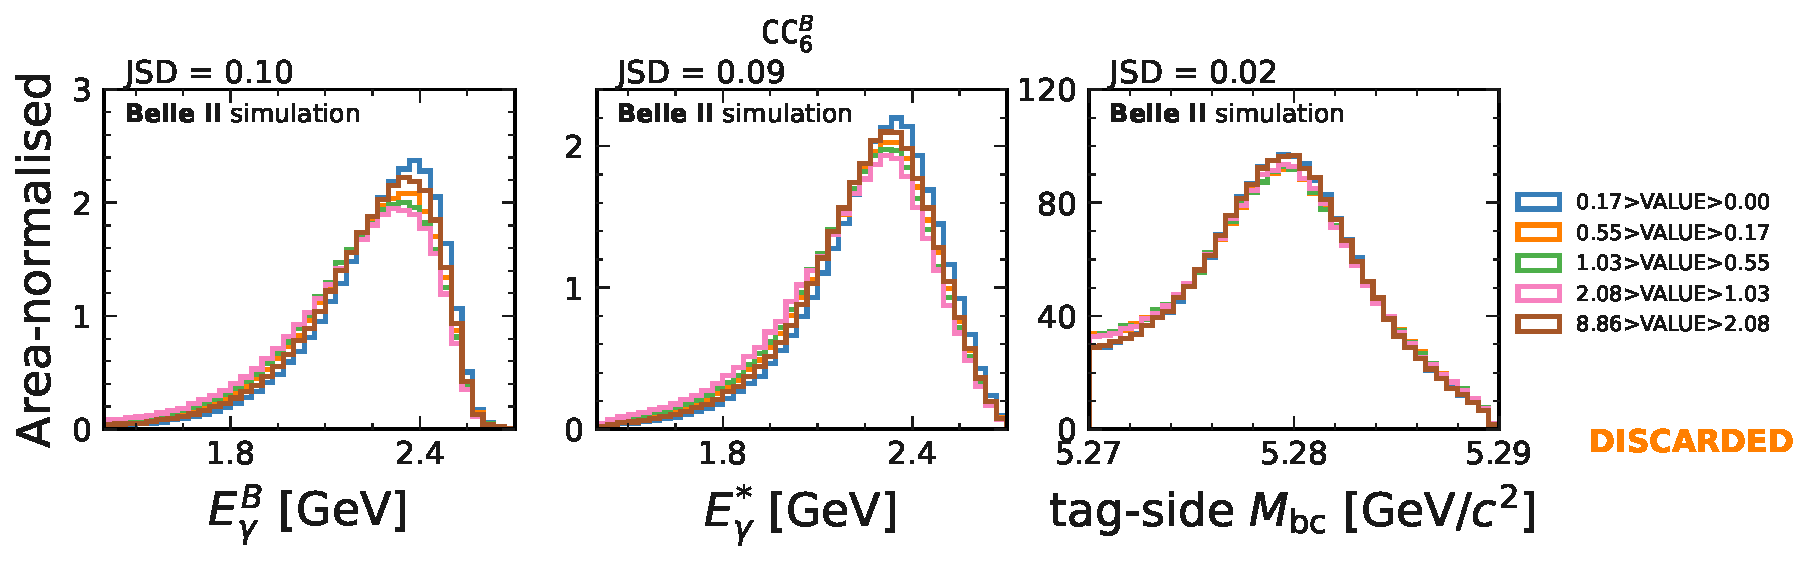
\includegraphics[width=0.95\textwidth]{figures/appendices/continuum_suppression_features/cleo_cones/Btag_CleoCone7_bias_tested.pdf}

    }
    \subcaptionbox{\label{fig:Btag_CleoCone7}}{
        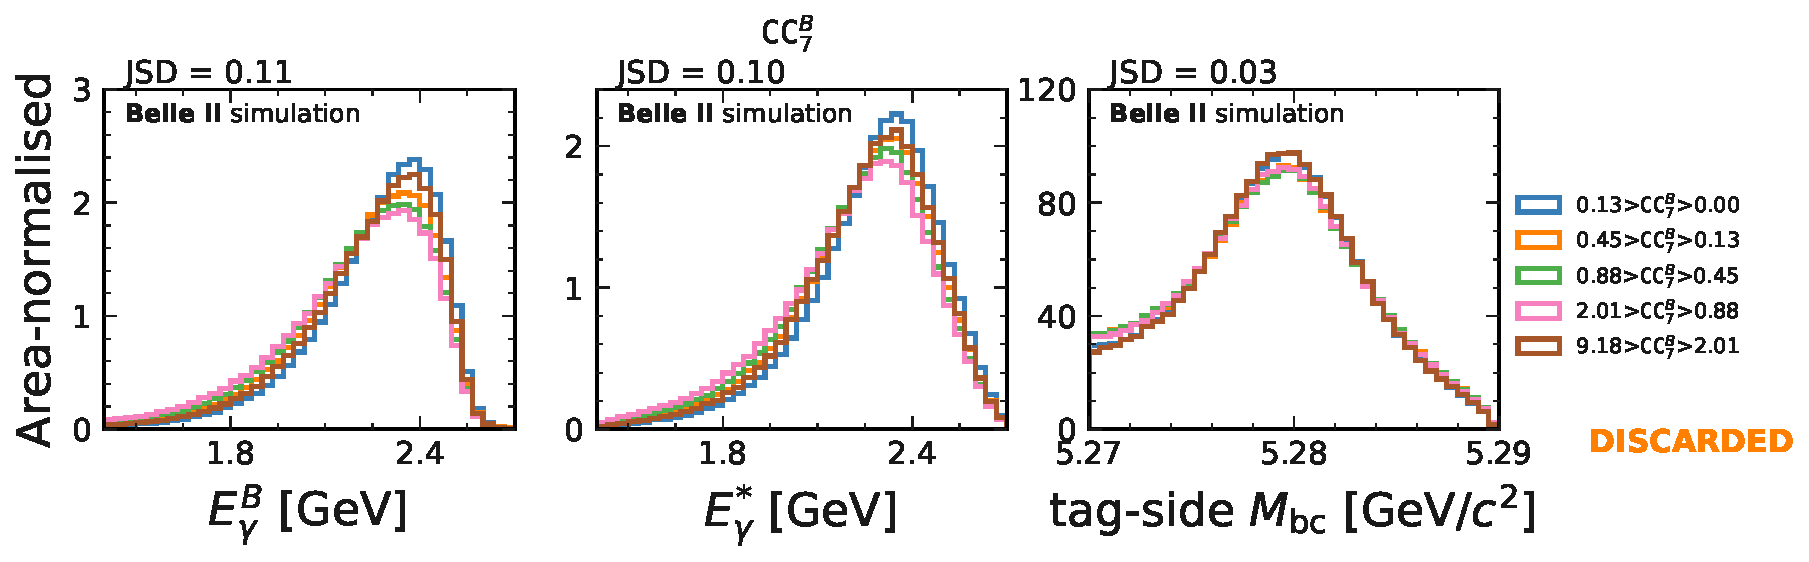
\includegraphics[width=0.95\textwidth]{figures/appendices/continuum_suppression_features/cleo_cones/Btag_CleoCone8_bias_tested.pdf}

    }
\end{figure}
\begin{figure}[htbp!]
\centering
\ContinuedFloat
    \subcaptionbox{\label{fig:Btag_CleoCone8}}{
        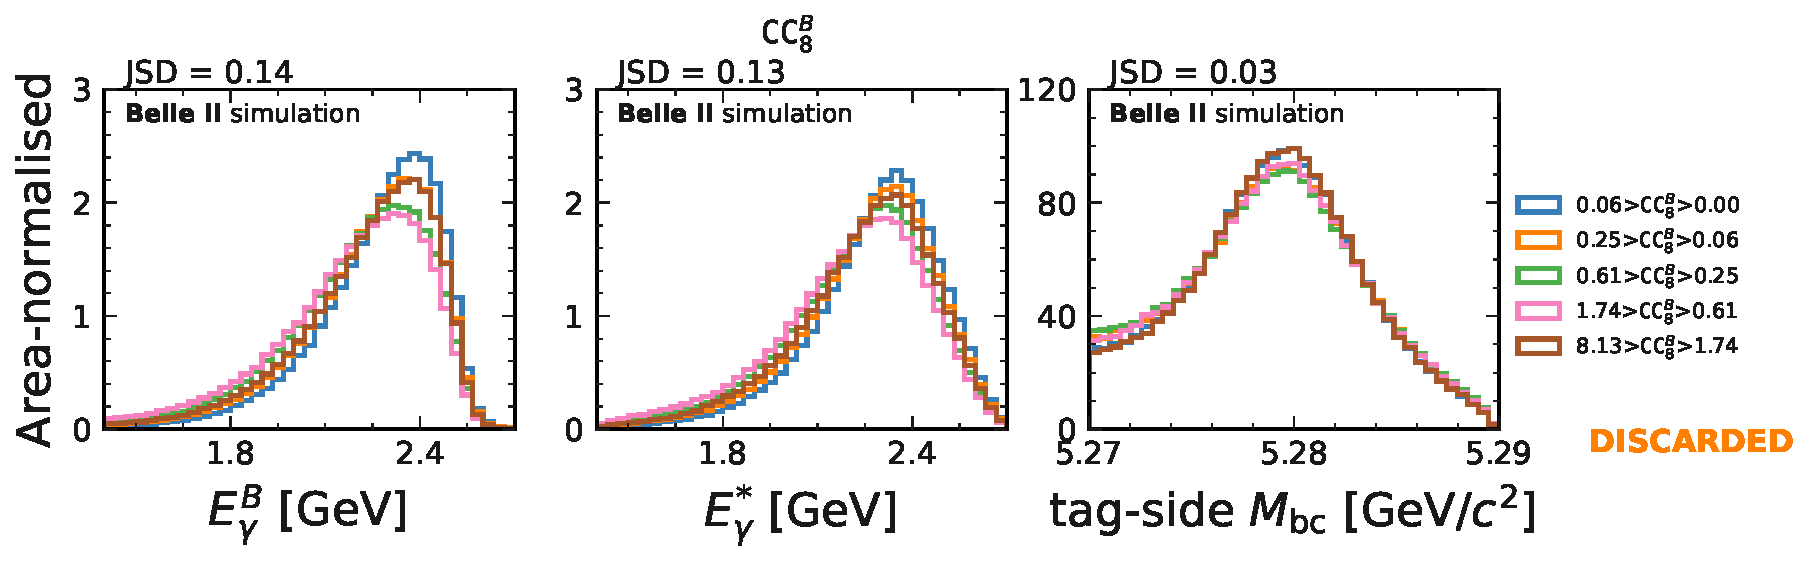
\includegraphics[width=0.95\textwidth]{figures/appendices/continuum_suppression_features/cleo_cones/Btag_CleoCone9_bias_tested.pdf}

    }
    \subcaptionbox{\label{fig:cleoConeThrust0}}{
        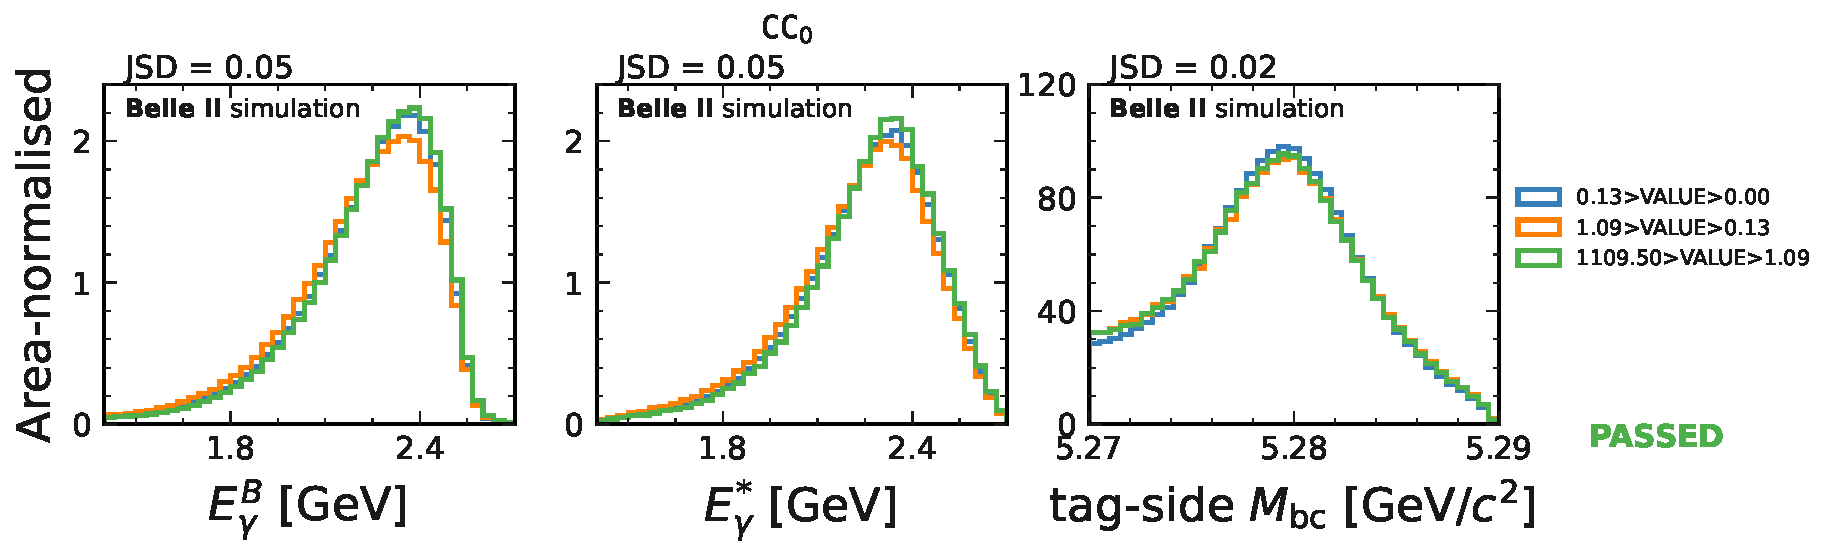
\includegraphics[width=0.95\textwidth]{figures/appendices/continuum_suppression_features/cleo_cones/cleoConeThrust0_bias_tested.pdf}

    }
    \subcaptionbox{\label{fig:cleoConeThrust1}}{
        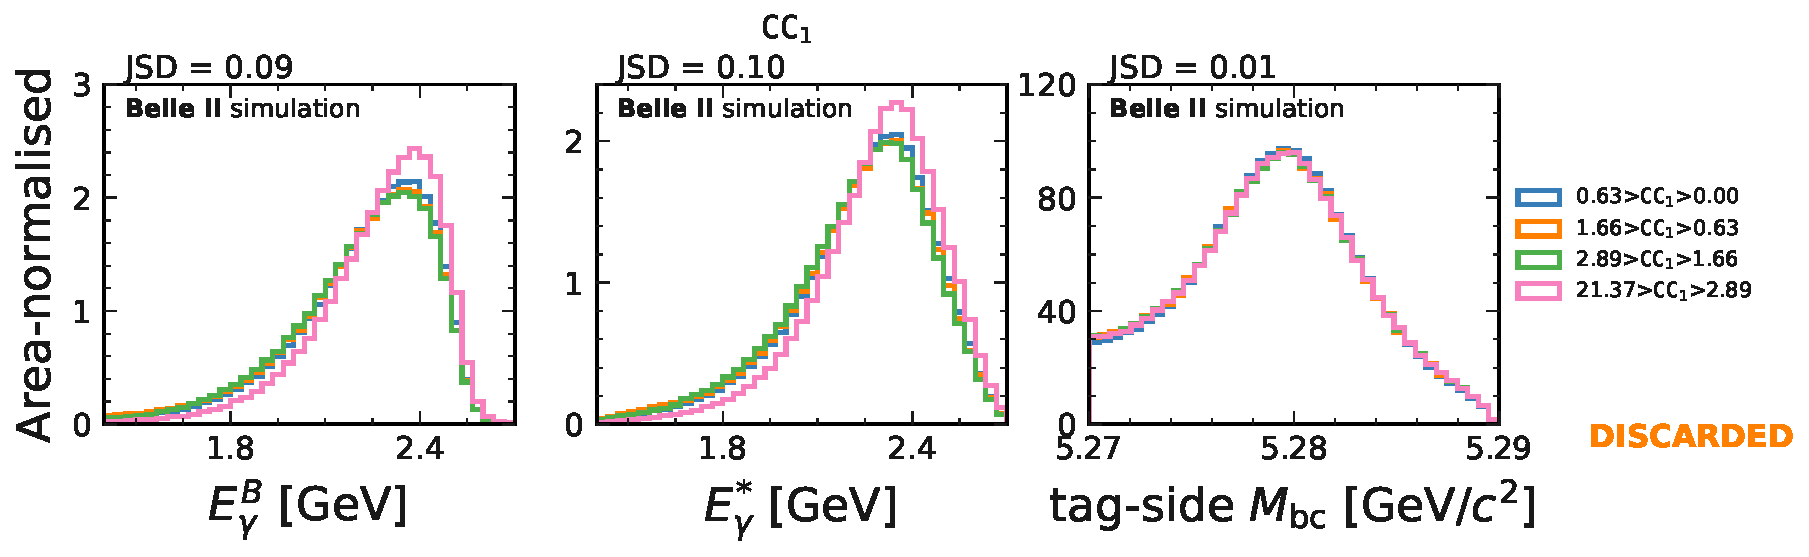
\includegraphics[width=0.95\textwidth]{figures/appendices/continuum_suppression_features/cleo_cones/cleoConeThrust1_bias_tested.pdf}

    }
    \subcaptionbox{\label{fig:cleoConeThrust2}}{
        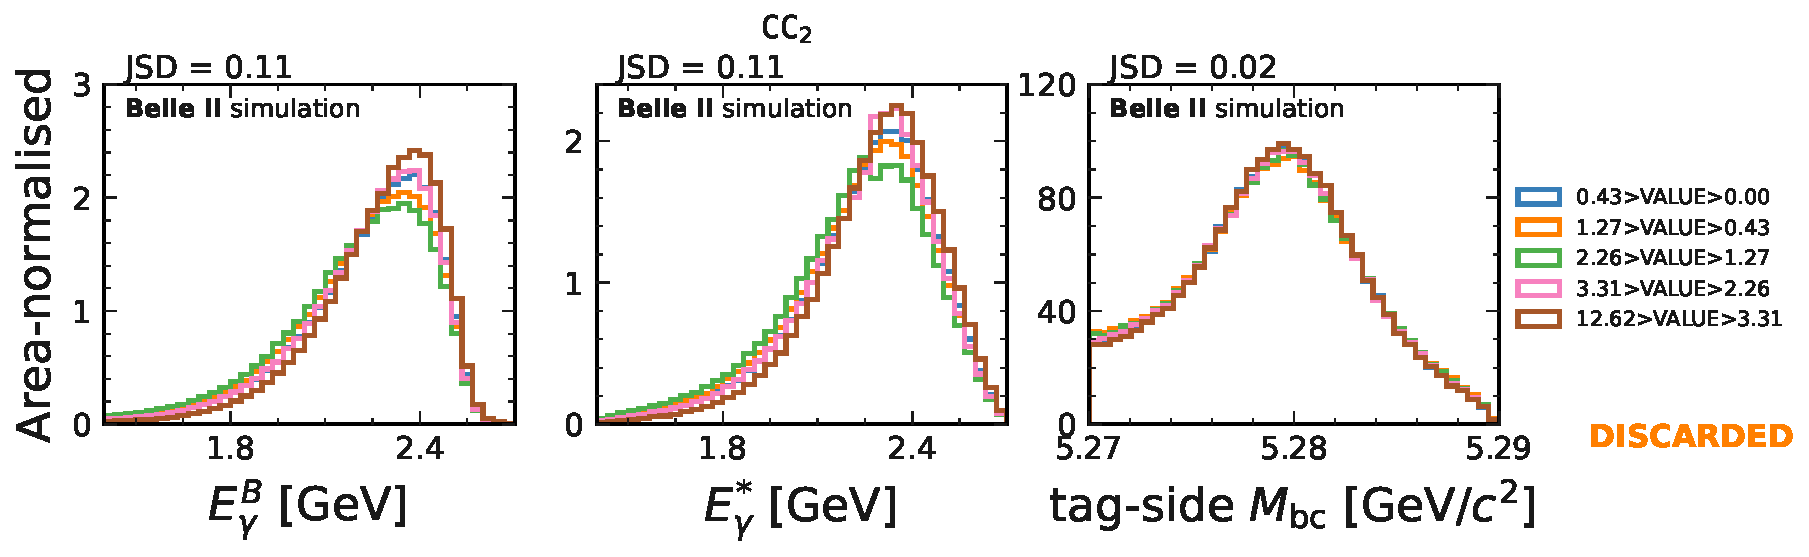
\includegraphics[width=0.95\textwidth]{figures/appendices/continuum_suppression_features/cleo_cones/cleoConeThrust2_bias_tested.pdf}

    }
\end{figure}
\begin{figure}[htbp!]
    \centering
    \ContinuedFloat
    \subcaptionbox{\label{fig:cleoConeThrust3}}{
        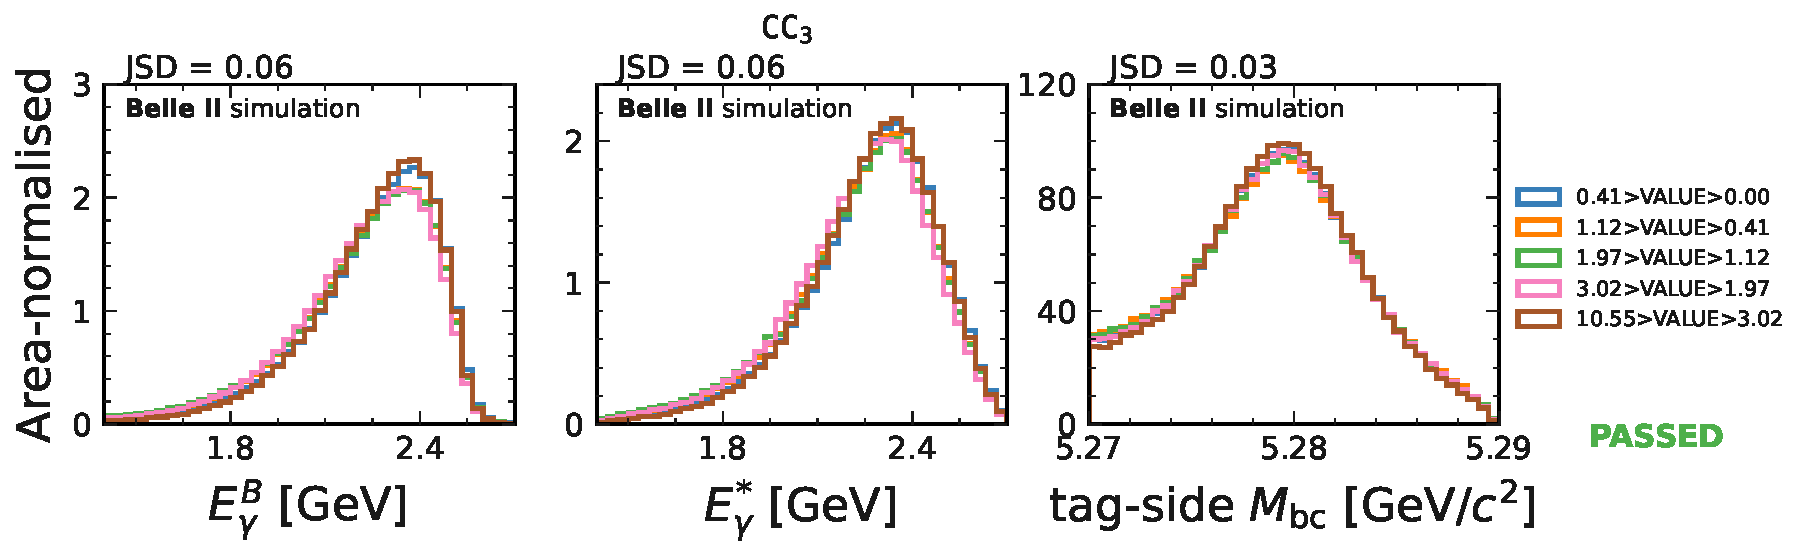
\includegraphics[width=0.95\textwidth]{figures/appendices/continuum_suppression_features/cleo_cones/cleoConeThrust3_bias_tested.pdf}

    }
    \subcaptionbox{\label{fig:cleoConeThrust4}}{
        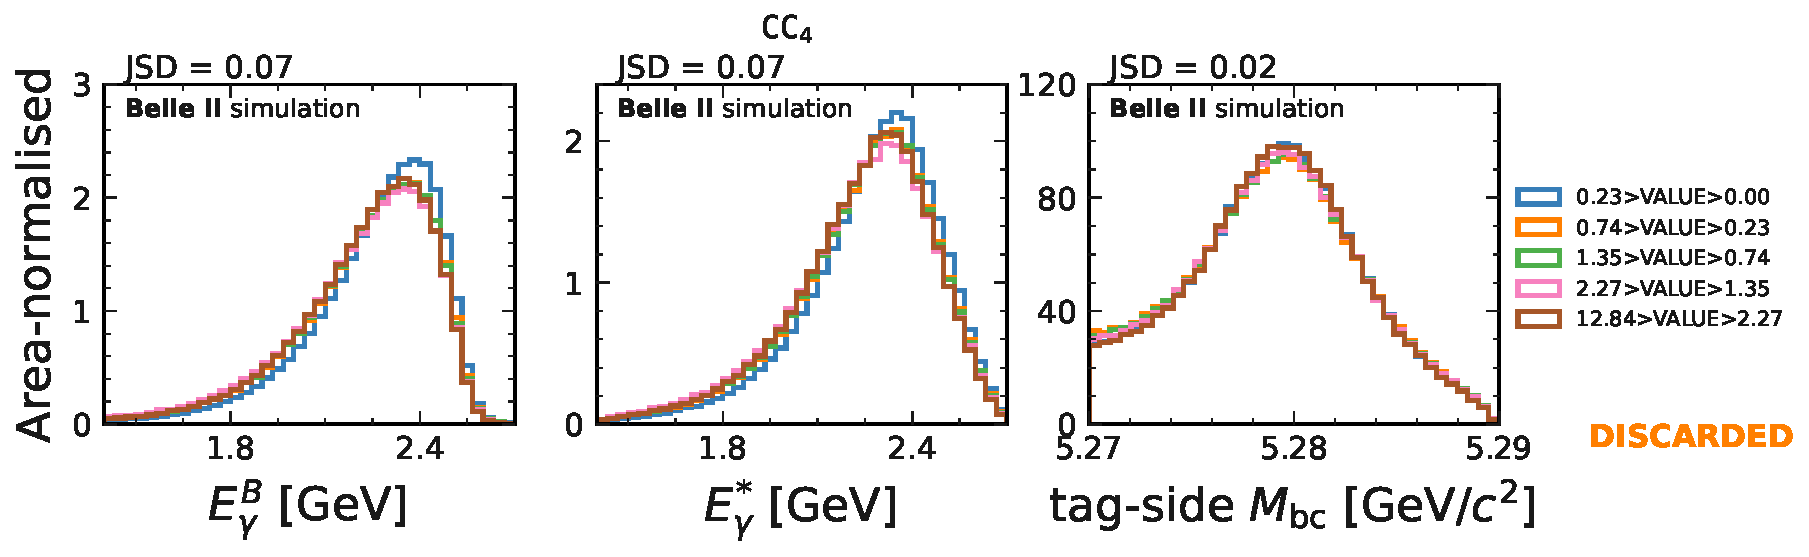
\includegraphics[width=0.95\textwidth]{figures/appendices/continuum_suppression_features/cleo_cones/cleoConeThrust4_bias_tested.pdf}

    }
    \subcaptionbox{\label{fig:cleoConeThrust5}}{
        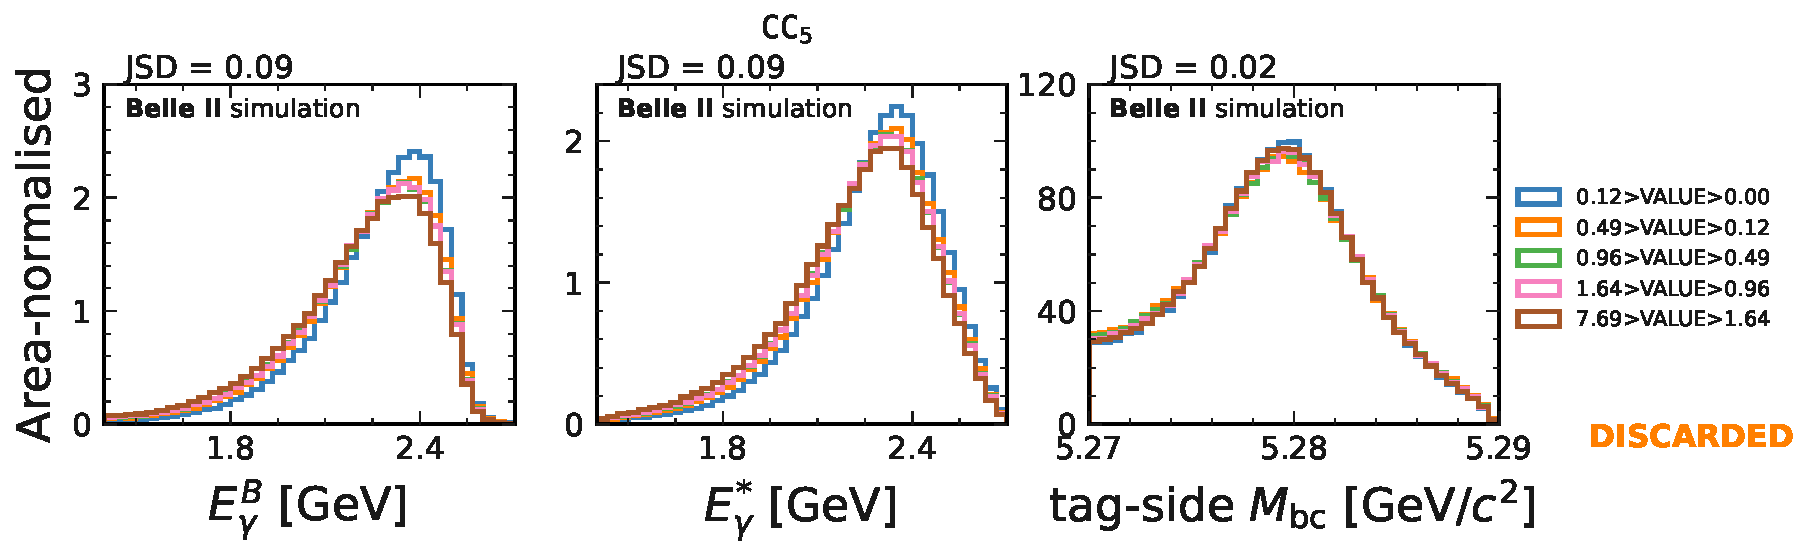
\includegraphics[width=0.95\textwidth]{figures/appendices/continuum_suppression_features/cleo_cones/cleoConeThrust5_bias_tested.pdf}

    }
    \subcaptionbox{\label{fig:cleoConeThrust6}}{
        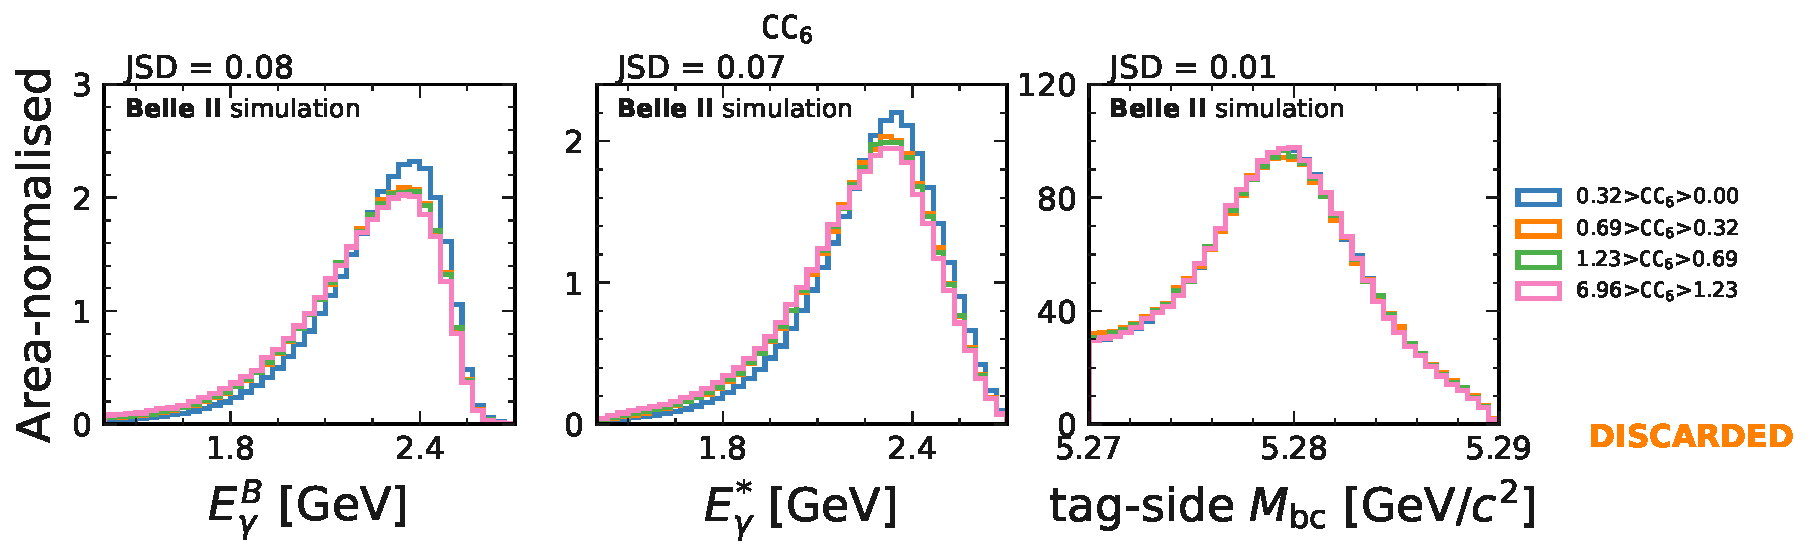
\includegraphics[width=0.95\textwidth]{figures/appendices/continuum_suppression_features/cleo_cones/cleoConeThrust6_bias_tested.pdf}

    }

\end{figure}
\begin{figure}[htbp!]
    \centering
    \ContinuedFloat
\subcaptionbox{\label{fig:cleoConeThrust7}}{
    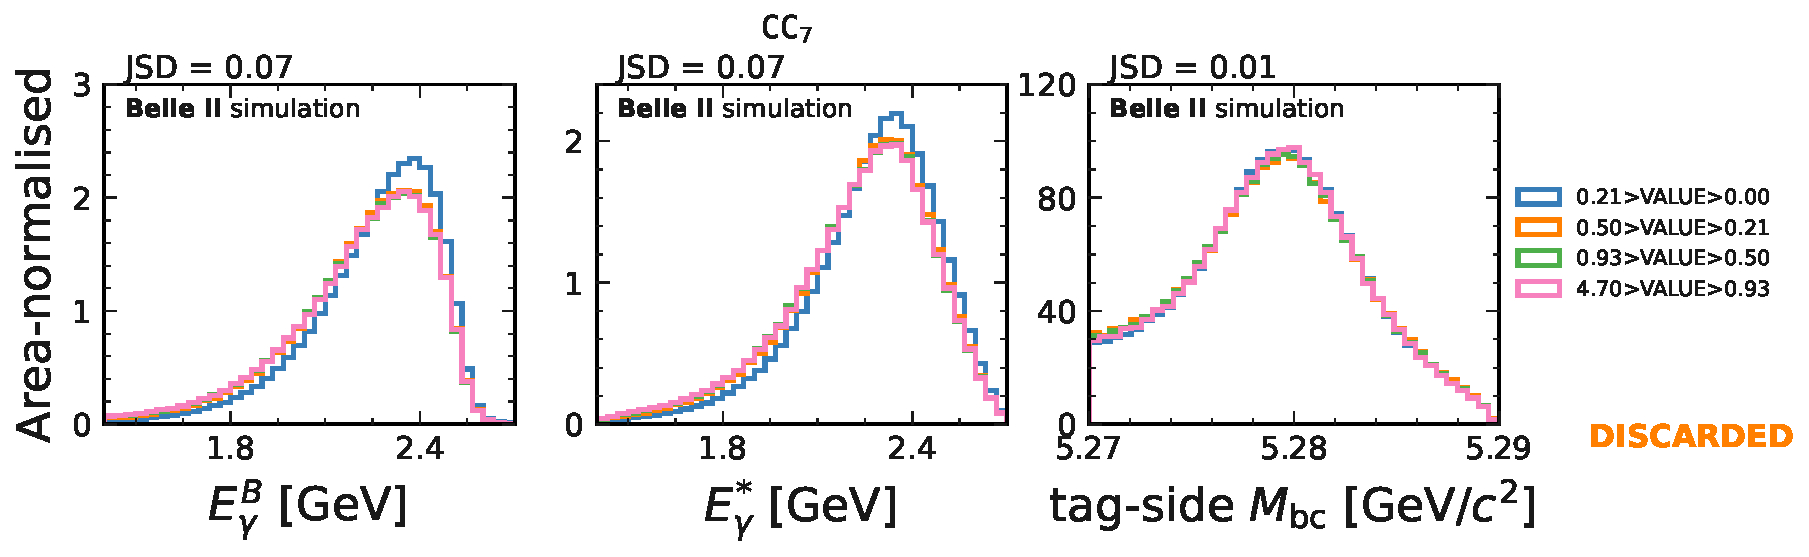
\includegraphics[width=0.95\textwidth]{figures/appendices/continuum_suppression_features/cleo_cones/cleoConeThrust7_bias_tested.pdf}

}
\subcaptionbox{\label{fig:cleoConeThrust8}}{
    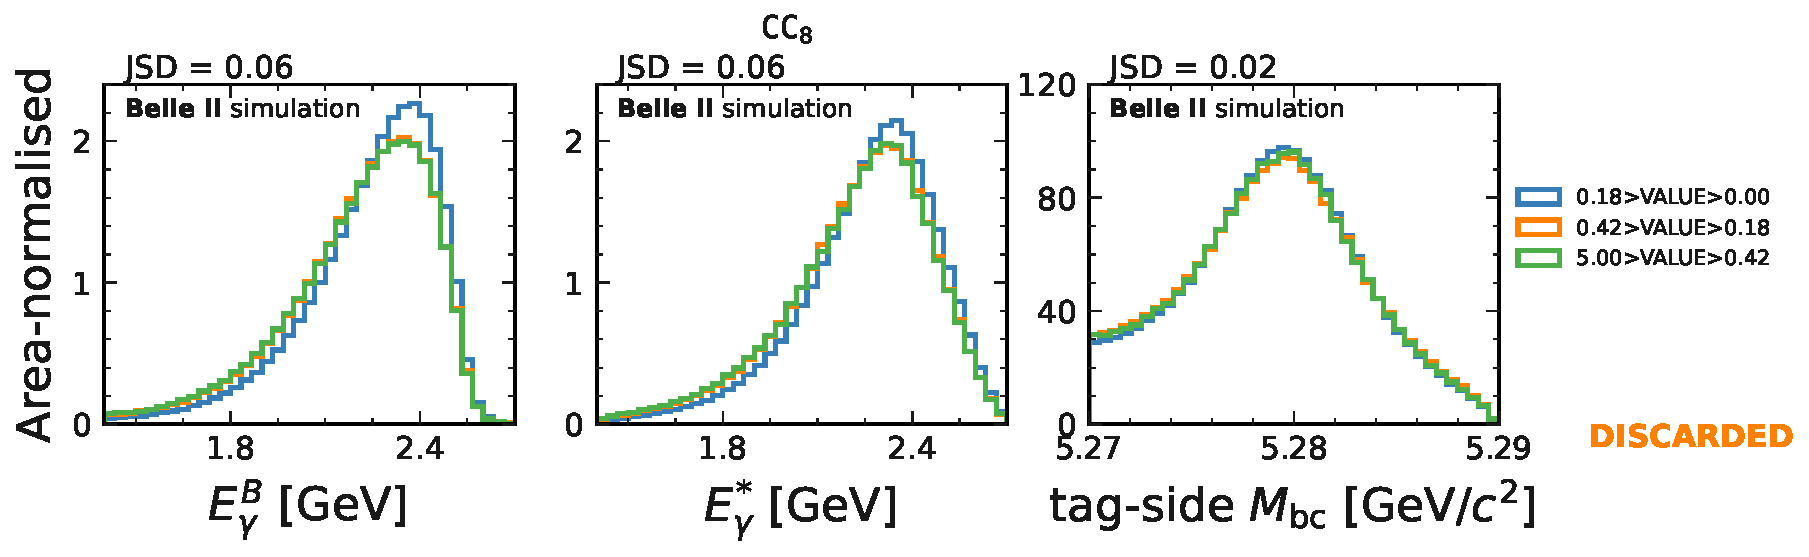
\includegraphics[width=0.95\textwidth]{figures/appendices/continuum_suppression_features/cleo_cones/cleoConeThrust8_bias_tested.pdf}

}
\caption{\label{fig:cleo_cones_test1} The bias-test on \EB, \Estar and \Mbc for modified Fox-Wolfram moments.
The test is performed based on \textbf{Test~1} strategy, defined in \Cref{sec:continuum_features}.
Variable definitions are given in the text.
The Jensen Shannon distance as introduced in \Cref{eq:js_distance} is given for each distribution.
}
\end{figure}
